\documentclass{article}

% PACKAGES for math, chemistry, layout, and graphics
\usepackage[a4paper, margin=1in]{geometry} % Sets page margins
\usepackage{amsmath}                      % For advanced math environments
\usepackage{graphicx}                     % To include images
\usepackage{pgfplots}                     % For creating plots and graphs
\usepackage{tikz}                         % For drawing diagrams
\usepackage[version=4]{mhchem}            % For typesetting chemical formulas (e.g., \ce{^{26}Cl})
\usepackage{hyperref}                     % For clickable links (optional)

% PGFPLOTS settings
\pgfplotsset{compat=1.17} % Use a recent compatibility version for pgfplots

% TIKZ library for positioning nodes
\usetikzlibrary{positioning}

% DOCUMENT TITLE
\title{A One-Hour Lesson on Radioactivity (Revised)}
\author{Gemini}
\date{\today}

\begin{document}

\maketitle

\section{Key Concepts in Radioactivity}
This section covers the essential principles needed to understand radioactive decay processes.

\subsection{Radioactive Decay and Half-Life}
Radioactivity is the process by which an unstable atomic nucleus loses energy by emitting radiation. The rate of this decay is exponential.

\begin{itemize}
    \item \textbf{Decay Equation:} The number of radioactive nuclei, $N$, at a given time, $t$, is described by the formula:
    \begin{equation}
        N(t) = N_0 e^{-\lambda t}
    \end{equation}
    Where $N_0$ is the initial number of nuclei and $\lambda$ is the decay constant.

    \item \textbf{Half-Life ($t_{1/2}$):} This is the time required for half of the radioactive nuclei in a sample to decay. It is the most common way to express the decay rate of an isotope.
\end{itemize}

% --- Exponential Decay Graph ---
\begin{figure}[h!]
\centering
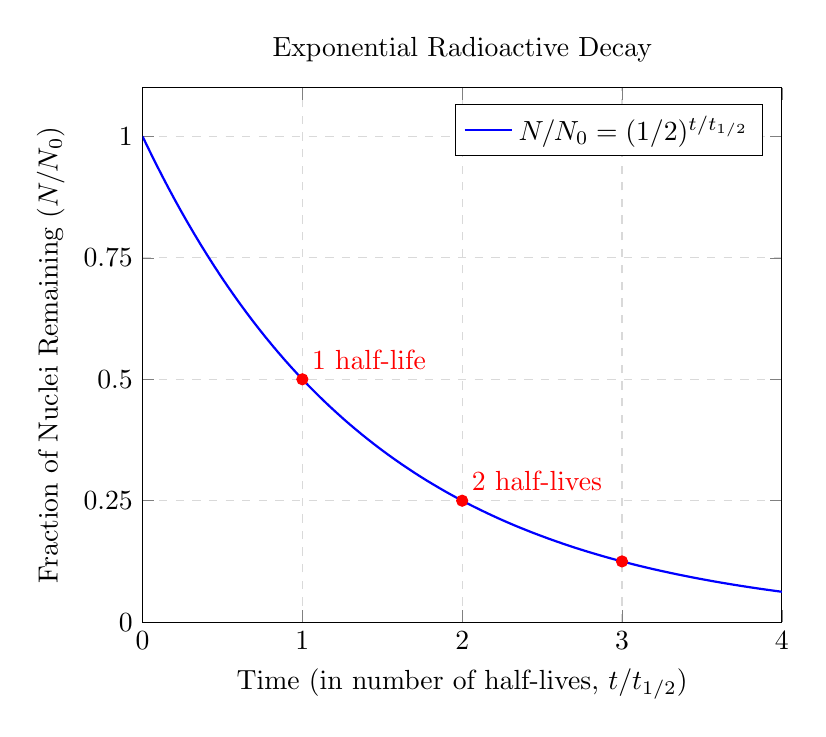
\begin{tikzpicture}
\begin{axis}[
    title={Exponential Radioactive Decay},
    xlabel={Time (in number of half-lives, $t/t_{1/2}$)},
    ylabel={Fraction of Nuclei Remaining ($N/N_0$)},
    xmin=0, xmax=4,
    ymin=0, ymax=1.1,
    xtick={0,1,2,3,4},
    ytick={0, 0.25, 0.5, 0.75, 1},
    legend pos=north east,
    grid=major,
    grid style={dashed,gray!30},
    width=0.8\textwidth,
]
\addplot[
    domain=0:4,
    samples=100,
    color=blue,
    thick,
]
{2^(-x)};
\addlegendentry{$N/N_0 = (1/2)^{t/t_{1/2}}$}

% Mark points for half-lives
\addplot[only marks, mark=*, color=red] coordinates {(1,0.5) (2,0.25) (3,0.125)};
\node[above right, red] at (axis cs:1,0.5) {1 half-life};
\node[above right, red] at (axis cs:2,0.25) {2 half-lives};

\end{axis}
\end{tikzpicture}
\caption{A graph showing the fraction of radioactive nuclei decreasing over time.}
\label{fig:decay_curve}
\end{figure}

\subsection{Decay Constant and Activity}
These two quantities provide a more fundamental description of the decay process.

\begin{itemize}
    \item \textbf{Decay Constant ($\lambda$):} This constant represents the probability of a single nucleus decaying per unit of time. It is inversely related to the half-life.
    \begin{equation}
        \lambda = \frac{\ln(2)}{t_{1/2}}
    \end{equation}
    
    \item \textbf{Activity (A):} This is the rate at which nuclei in a sample decay. Since the number of nuclei $N$ decreases over time, its rate of change $\frac{dN}{dt}$ is negative, representing the exponential decay.
    \begin{equation}
        \frac{dN}{dt} = - \lambda N
    \end{equation}
    Activity is defined as the magnitude of this rate (a positive value), measured in Becquerels (Bq), where 1 Bq = 1 decay per second.
    \begin{equation}
        A = -\frac{dN}{dt} = \lambda N
    \end{equation}
    Like the number of nuclei, activity also decreases exponentially over time: $A(t) = A_0 e^{-\lambda t}$.
\end{itemize}

\subsection{Decay Series and Branching}
Nuclei can decay through complex pathways.

\begin{itemize}
    \item \textbf{Serial Decay (Decay Chain):} This occurs when a radioactive nucleus (parent, A) decays into another radioactive nucleus (daughter, B), which in turn decays to a stable nucleus (C).
    \[ \ce{A ->[\lambda_A] B ->[\lambda_B] C} \]
    The quantity of the intermediate nucleus B first increases and then decreases.
\end{itemize}
% --- Serial Decay Graph ---
\begin{figure}[h!]
\centering
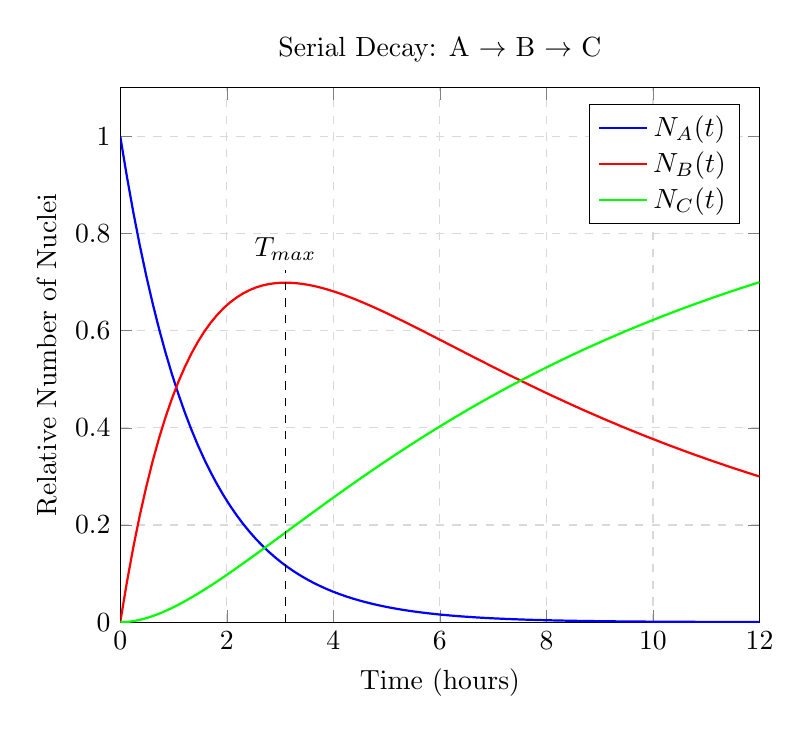
\begin{tikzpicture}
\begin{axis}[
    title={Serial Decay: A $\to$ B $\to$ C},
    xlabel={Time (hours)},
    ylabel={Relative Number of Nuclei},
    xmin=0, xmax=12,
    ymin=0, ymax=1.1,
    legend pos=north east,
    grid=major,
    grid style={dashed,gray!30},
    width=0.8\textwidth,
]
% Define decay constants from Problem 1 for plotting
\def\lambdaA{0.693}
\def\lambdaB{0.1155}

% Plot for Nucleus A
\addplot[domain=0:12, samples=100, color=blue, thick] {exp(-\lambdaA*x)};
\addlegendentry{$N_A(t)$}

% Plot for Nucleus B
\addplot[domain=0:12, samples=100, color=red, thick] {(\lambdaA/(\lambdaB-\lambdaA)) * (exp(-\lambdaA*x) - exp(-\lambdaB*x))};
\addlegendentry{$N_B(t)$}

% Plot for Nucleus C
\addplot[domain=0:12, samples=100, color=green, thick] {1 - ((\lambdaB*exp(-\lambdaA*x) - \lambdaA*exp(-\lambdaB*x))/(\lambdaB-\lambdaA))};
\addlegendentry{$N_C(t)$}

% Add a vertical line for T_max
\draw[dashed, black] (axis cs:3.10,0) -- (axis cs:3.10,0.725);
\node[above] at (axis cs:3.10, 0.725) {$T_{max}$};
\end{axis}
\end{tikzpicture}
\caption{Graph showing the relative quantities of nuclei A, B, and C in a decay chain.}
\label{fig:serial_decay}
\end{figure}

\subsubsection*{Derivation of the Serial Decay Equation for Intermediate Nucleus B}
The number of nuclei of the intermediate isotope, B, changes based on its rate of formation from A and its own rate of decay into C.
\begin{enumerate}
    \item The rate of formation of B is equal to the activity of A: $\lambda_A N_A(t)$.
    \item The rate of decay of B is equal to its own activity: $\lambda_B N_B(t)$.
    \item The net rate of change of B is the difference between these two rates:
    \begin{equation*}
        \frac{dN_B}{dt} = (\text{Rate of formation}) - (\text{Rate of decay}) = \lambda_A N_A(t) - \lambda_B N_B(t)
    \end{equation*}
    \item We know that $N_A(t) = N_{A,0} e^{-\lambda_A t}$. Substituting this in gives:
    \begin{equation*}
        \frac{dN_B}{dt} = \lambda_A N_{A,0} e^{-\lambda_A t} - \lambda_B N_B(t)
    \end{equation*}
    \item Rearranging this equation into the standard form of a first-order linear differential equation gives:
    \begin{equation*}
        \frac{dN_B}{dt} + \lambda_B N_B(t) = \lambda_A N_{A,0} e^{-\lambda_A t}
    \end{equation*}
    \item This equation matches the general form provided in Problem 1, $\frac{dy}{dx}+c_{1}y=c_{2}e^{-kx}$, with the following substitutions:
    \begin{itemize}
        \item $y \rightarrow N_B$
        \item $x \rightarrow t$
        \item $c_1 \rightarrow \lambda_B$
        \item $c_2 \rightarrow \lambda_A N_{A,0}$
        \item $k \rightarrow \lambda_A$
    \end{itemize}
    \item Plugging these into the provided solution, $y=\frac{c_{2}}{c_{1}-k}(e^{-kx}-e^{-c_{1}x})$, yields the final equation for $N_B(t)$, assuming $N_B(0)=0$:
    \begin{equation}
        N_B(t) = \frac{\lambda_A N_{A,0}}{\lambda_B - \lambda_A} (e^{-\lambda_A t} - e^{-\lambda_B t})
    \end{equation}
\end{enumerate}

\begin{itemize}
    \item \textbf{Branching Decay:} This is when a nucleus can decay through two or more different pathways. The total decay constant is the sum of the decay constants for each branch. The fraction of decays that proceed through a specific path is the \textbf{branching ratio}.
\end{itemize}

% --- Branching Decay Diagram ---
\begin{figure}[h!]
\centering
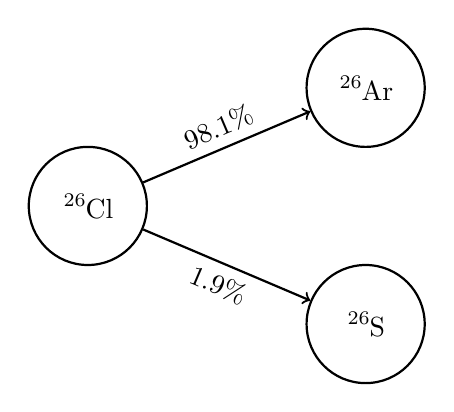
\begin{tikzpicture}[
    node distance=2cm,
    nuclide/.style={circle, draw=black, thick, minimum size=1.5cm, align=center}
]
    % Nodes for the nuclei
    \node[nuclide] (Cl) {\ce{^{26}Cl}};
    \node[nuclide, right=of Cl, yshift=1.5cm] (Ar) {\ce{^{26}Ar}};
    \node[nuclide, right=of Cl, yshift=-1.5cm] (S) {\ce{^{26}S}};
    
    % Arrows with probabilities
    \draw[->, thick] (Cl) -- (Ar) node[midway, above, sloped] {98.1\%};
    \draw[->, thick] (Cl) -- (S) node[midway, below, sloped] {1.9\%};
\end{tikzpicture}
\caption{Branching decay of \ce{^{26}Cl}.}
\label{fig:branching_decay}
\end{figure}

\newpage
\section{Problem Solving \& Solutions}

\subsection*{Problem 1 (from Nuclear1.pdf)}
\textbf{Question:} \textit{Radioactive nucleus A with a half-life of 1 hour decays into another radioactive nucleus B which has a half-life of 6 hours. Nucleus B decays into nucleus C which is stable. At time t=0, a specimen contains $10^{-3}$ mole of A but none of B and C. Nucleus B in the specimen reaches a maximum quantity of X nuclei at time t=T hours. Find X and T.}

\subsubsection*{Solution}
This is a serial decay problem (A $\longrightarrow$ B $\longrightarrow$ C).
\begin{enumerate}
    \item \textbf{Calculate the decay constants ($\lambda$) for A and B:}
    \begin{align*}
        \lambda_A &= \frac{\ln(2)}{t_{1/2, A}} = \frac{\ln(2)}{1 \text{ hr}} = 0.693 \text{ hr}^{-1} \\
        \lambda_B &= \frac{\ln(2)}{t_{1/2, B}} = \frac{\ln(2)}{6 \text{ hr}} = 0.1155 \text{ hr}^{-1}
    \end{align*}

    \item \textbf{Find the time, T, for maximum quantity of B:}
    The maximum occurs when $\frac{dN_B}{dt}=0$. As shown in the derivation, this means the rate of formation equals the rate of decay: $\lambda_A N_A(T) = \lambda_B N_B(T)$. This leads to the formula:
    \begin{equation*}
        T = \frac{\ln(\lambda_A / \lambda_B)}{\lambda_A - \lambda_B} = \frac{\ln(0.693 / 0.1155)}{0.693 - 0.1155} = \frac{\ln(6)}{0.5775} \approx \mathbf{3.10 \textbf{ hours}}
    \end{equation*}

    \item \textbf{Calculate the maximum quantity of B nuclei, X:}
    First, find the initial number of A nuclei, $N_{A,0}$:
    \begin{equation*}
        N_{A,0} = (10^{-3} \text{ mol}) \times (6.022 \times 10^{23} \text{ mol}^{-1}) = 6.022 \times 10^{20} \text{ nuclei}
    \end{equation*}
    Now, substitute $t=T=3.10$ hours into the equation for $N_B(t)$ (Equation 5):
    \begin{align*}
        X = N_B(3.10) &= \frac{0.693 \times (6.022 \times 10^{20})}{0.1155 - 0.693} (e^{-0.693 \times 3.10} - e^{-0.1155 \times 3.10}) \\
        X &= \frac{4.173 \times 10^{20}}{-0.5775} (0.1167 - 0.699) \\
        X &= -7.226 \times 10^{20} (-0.5823) \approx \mathbf{4.21 \times 10^{20} \textbf{ nuclei}}
    \end{align*}
\end{enumerate}

\hrulefill

\subsection*{Problem 2 (from Nuclear3.pdf)}
\textbf{Question:} \textit{Consider the radioisotope \ce{^{26}Cl}. \ce{^{26}Cl} decays with 98.1\% probability to \ce{^{26}Ar} and with 1.9\% probability to \ce{^{26}S}. In a sample of old groundwater, the masses of \ce{^{26}Cl} and \ce{^{26}S} were measured to be 20 µg and 0.36 µg respectively. The age of this water was deduced to be 290,000 years. Find the half-life of \ce{^{26}Cl}.}

\subsubsection*{Solution}
This problem involves branching decay. The mass of \ce{^{26}S} produced is 1.9\% of the total mass of \ce{^{26}Cl} that has decayed.
\begin{enumerate}
    \item \textbf{Find the initial mass of \ce{^{26}Cl} ($m_{Cl,0}$):}
    \begin{align*}
        m_S(t) &= (m_{Cl,0} - m_{Cl}(t)) \times (\text{Branching Ratio}) \\
        0.36 \text{ µg} &= (m_{Cl,0} - 20 \text{ µg}) \times 0.019 \\
        m_{Cl,0} &= \frac{0.36}{0.019} + 20 = 18.95 + 20 = 38.95 \text{ µg}
    \end{align*}

    \item \textbf{Calculate the decay constant ($\lambda$):}
    \begin{align*}
        m_{Cl}(t) &= m_{Cl,0} e^{-\lambda t} \\
        20 &= 38.95 \times e^{-\lambda \times 290000} \\
        \ln\left(\frac{20}{38.95}\right) &= -290000\lambda \\
        -0.6665 &= -290000\lambda \\
        \lambda &= \frac{0.6665}{290000} \approx 2.298 \times 10^{-6} \text{ years}^{-1}
    \end{align*}

    \item \textbf{Calculate the half-life ($t_{1/2}$):}
    \begin{equation*}
        t_{1/2} = \frac{\ln(2)}{\lambda} = \frac{0.693}{2.298 \times 10^{-6}} \approx 301,566 \text{ years}
    \end{equation*}
    The half-life of \ce{^{26}Cl} is approximately \textbf{302,000 years}.
\end{enumerate}

\hrulefill

\subsection*{Problem 3 (from Nuclear2.pdf)}
\textbf{Question:} \textit{A 5.00 ml solution was injected into the bloodstream of a patient. The solution contains radioactive iodine \ce{^{131}I} with a half-life of 8.025 days at a concentration of $1.00 \times 10^{-10} kgm^{-3}$. The activity of a 5.00 ml blood sample taken 24 hours later is found to be 3171 counts in 30 minutes. (a) Calculate the decay constant. (b) Calculate the total volume of blood in the patient's body.}

\subsubsection*{Solution}
\begin{enumerate}
    \item[\textbf{(a)}] \textbf{Calculate the decay constant ($\lambda$):}
    \begin{align*}
        t_{1/2} &= 8.025 \text{ days} = 8.025 \times 24 \times 3600 \text{ s} = 6.9336 \times 10^5 \text{ s} \\
        \lambda &= \frac{\ln(2)}{t_{1/2}} = \frac{0.6931}{6.9336 \times 10^5 \text{ s}} \approx \mathbf{1.00 \times 10^{-6} \textbf{ s}^{-1}}
    \end{align*}

    \item[\textbf{(b)}] \textbf{Calculate the total blood volume:}
    \begin{enumerate}
        \item \textit{Initial number of nuclei injected ($N_0$):}
        \begin{align*}
            m_{inj} &= (1.00 \times 10^{-10} \text{ kg/m}^3) \times (5.00 \times 10^{-6} \text{ m}^3) = 5.00 \times 10^{-16} \text{ kg} \\
            N_0 &= \frac{m_{inj}}{\text{Molar Mass}} \times N_A = \frac{5.00 \times 10^{-16} \text{ kg}}{0.131 \text{ kg/mol}} \times (6.022 \times 10^{23} \text{ mol}^{-1}) \approx 2.298 \times 10^9 \text{ nuclei}
        \end{align*}

        \item \textit{Nuclei remaining after 24 hours ($N(t)$):}
        \begin{align*}
            \lambda_{\text{days}} &= \frac{\ln(2)}{8.025 \text{ days}} \approx 0.08637 \text{ days}^{-1} \\
            N(t) &= N_0 e^{-\lambda t} = (2.298 \times 10^9) \times e^{-0.08637 \times 1} \approx 2.108 \times 10^9 \text{ nuclei}
        \end{align*}

        \item \textit{Number of nuclei in the sample ($N_{sample}$):}
        \begin{align*}
            A_{sample} &= \frac{3171 \text{ counts}}{30 \times 60 \text{ s}} = 1.7617 \text{ Bq} \\
            N_{sample} &= \frac{A_{sample}}{\lambda} = \frac{1.7617 \text{ s}^{-1}}{1.00 \times 10^{-6} \text{ s}^{-1}} \approx 1.762 \times 10^6 \text{ nuclei}
        \end{align*}

        \item \textit{Total blood volume ($V_{blood}$):}
        Assuming uniform distribution: $\frac{N_{sample}}{V_{sample}} = \frac{N(t)}{V_{blood}}$
        \begin{equation*}
             V_{blood} = V_{sample} \times \frac{N(t)}{N_{sample}} = 5.00 \text{ ml} \times \frac{2.108 \times 10^9}{1.762 \times 10^6} \approx 5982 \text{ ml} \approx \mathbf{5.98 \textbf{ L}}
        \end{equation*}
    \end{enumerate}
    \textbf{Assumption:} The primary assumption is that the radioactive iodine becomes \textbf{uniformly distributed} throughout the patient's entire blood volume within the 24-hour period.
\end{enumerate}

\end{document}